\subsection{Code suggestion}
Another use of the knowledge graph could be to provide code suggestions for data scientists.  To evaluate the potential to use the knowledge graph for this use case, we evaluated how many data flow edge successors existed for path lengths of 1, 2, and 3 in test programs.  A path length of 1 assumes only one turtle call site had been written in the code, where a data scientist had made one API call to a data science library, and the question is how well we could predict the very next set of calls using the knowledge graph.  Similarly, path lengths of 2 and 3 model the case when the data scientist has written two or three API calls, and the question being asked is how many suggestions on average we would predict using the knowledge graph.  We note that this is a relatively naive way to use the knowledge graph for code completion, but we do so to evaluate the quality of the graph for the use case rather than suggesting that a code completion system be designed in this way. As before, we evaluated this using a 10 fold split of test programs, where we rotated each set as the `test' case, and used the remaining nine sets to model the knowledge graph we could query against.  

\begin{figure}
\centering 
{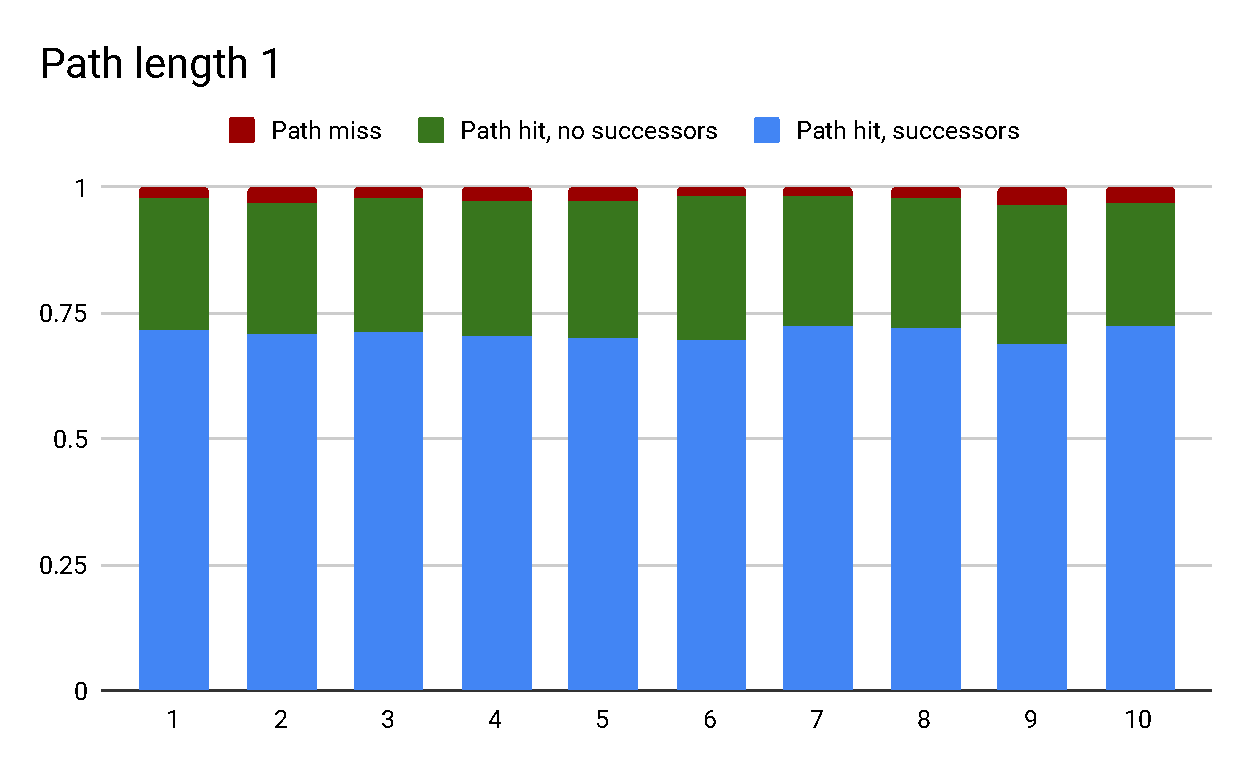
\includegraphics[width=0.4\textwidth]{path_length_1}}%
\hfill 
{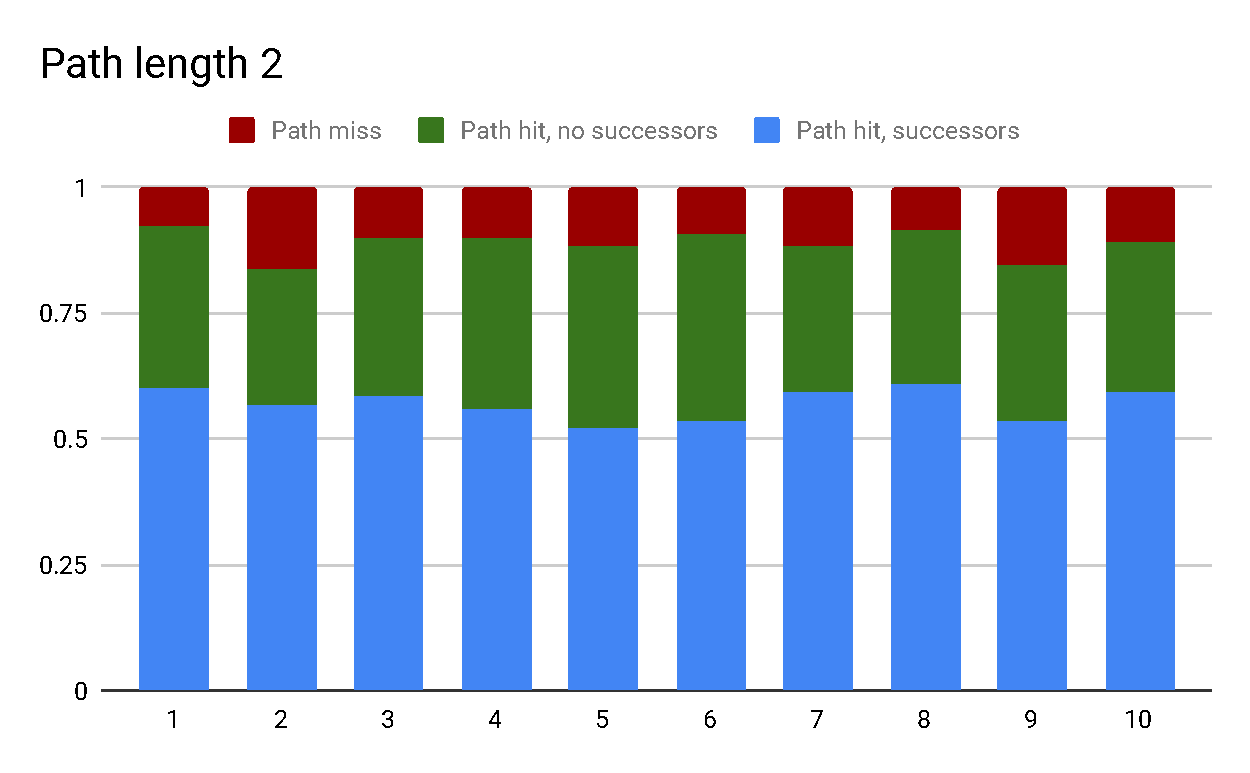
\includegraphics[width=0.4\textwidth]{path_length_2}}%
\hfill 
{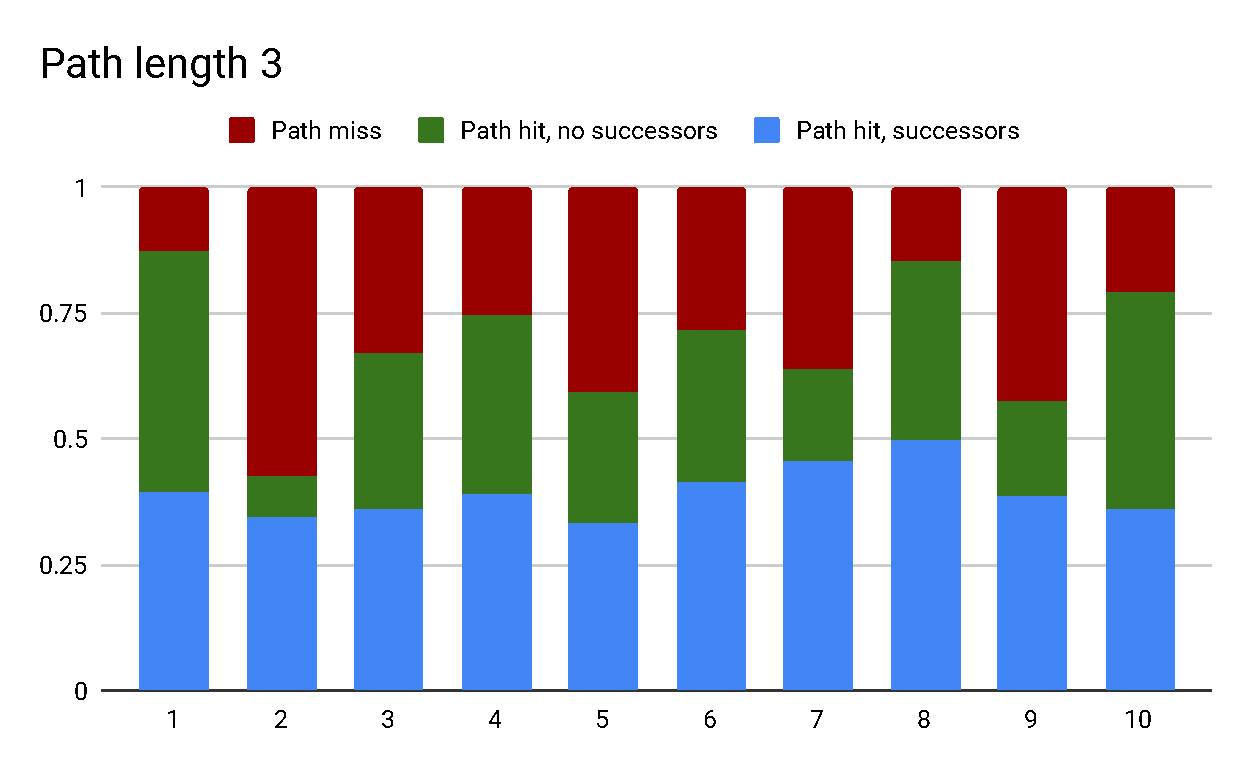
\includegraphics[width=0.4\textwidth]{path_length_3}}%
\caption{Path lengths of 1, 2 and 3}
\label{cross_validate_paths}
\end{figure}

Figure~\ref{cross_validate_paths} shows the percentage of paths in the test programs of length 1, 2 and 3 we found in the knowledge graph across the 10 splits.  As shown in the figure, when we were able to find 97.5\% of paths of length 1 in the knowledge graph, 88.9\% of paths of length 2, and 68.9\% of paths of length 3.  Of those, 71.1\% of paths of length 1 had successors, 57.1\% of paths of length 2 had successors, and 39.5\% of paths of length 3 had successors.  Figure~\ref{cross_validate_means} shows the average number of successors for different path lengths across the 10 runs.  The average number of successors across runs was 176.5 for paths of length 1, 49.9 for paths of length 2, 7.3 for paths of length 3. 

\begin{figure}
\centering  
{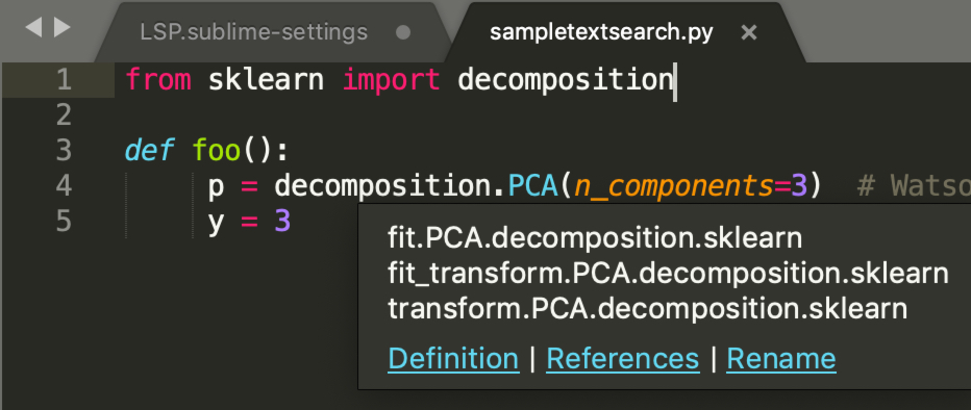
\includegraphics[width=0.45\textwidth]{sublime}}
\caption{Code suggestions in Sublime Text 3}
\label{code_suggestion_ide}
\end{figure}
  
While there are many enhancements that could improve an actual code suggestion system---e.g., considering control flow edges to prune successors, analyzing if objects exist that could flow into parameters that are needed for successors, etc., these results suggest that with sufficient context (i.e., more API calls written by the user to infer intent), the knowledge graph can actually be used provide a small enough number of successors as suggestions.  To make this concrete, in Figure~\ref{code_suggestion_ide}, we show a screenshot of prototype code suggestions in Sublime Text 3 based on our knowledge graph.  The user hovers over the {\tt PCA.decomposition.sklearn} constructor, and the tool runs the SPARQL query in Figure~\ref{code:code_suggestion_sparql} on our knowledge graph after substituting {\tt PCA.decomposition.sklearn} for {\tt ?m}.   The query suggests {\tt fit} variants as something to do next, as that is what our graph shows is most common.

\begin{figure}[htb]
\begin{centering}
\lstinputlisting[language=Python,escapechar=|]{./code_suggestion_sparql.txt}
\caption{SPARQL query for code suggestions}
\label{code:code_suggestion_sparql}
\end{centering}
\end{figure}

\begin{figure}
\centering 
{\includegraphics[width=0.5\textwidth]{avg_successors}}
\caption{Path lengths of 1, 2 and 3}
\label{cross_validate_means}
\end{figure}

